\documentclass{beamer}
\usepackage{pgfpages}
%\setbeameroption{show notes on second screen=left} %enable for notes
\usepackage{graphicx}
\usepackage{xcolor}
\usepackage{listings}
\usepackage{hyperref}
\lstset{language=python,frame=single}
\usepackage{verbatim}
\usepackage{subcaption}
\usepackage{amsmath}
\usepackage{relsize}
\usepackage{appendixnumberbeamer}
\usepackage{xparse}
\usepackage{multimedia}
\usepackage{tikz}
\usetikzlibrary{matrix,backgrounds}
\pgfdeclarelayer{myback}
\pgfsetlayers{myback,background,main}

\tikzset{mycolor/.style = {line width=1bp,color=#1}}%
\tikzset{myfillcolor/.style = {draw,fill=#1}}%
\tikzstyle{line} = [draw, line width=1pt]
\tikzstyle{arrow} = [draw, line width=1pt, ->]

\NewDocumentCommand{\highlight}{O{blue!40} m m}{%
\draw[mycolor=#1,rounded corners] (#2.north west)rectangle (#3.south east);
}

\NewDocumentCommand{\fhighlight}{O{blue!40} m m}{%
\draw[myfillcolor=#1,rounded corners] (#2.north west)rectangle (#3.south east);
}

\usetheme[numbering=fraction, background=dark]{metropolis}
%%\AtBeginSection[]
%%{
%%  \begin{frame}
%%    \frametitle{Table of Contents}
%%    \tableofcontents[currentsection]
%%  \end{frame}
%%}

%%\let\olditem\item
%%\renewcommand{\item}{\vspace{0.5\baselineskip}\olditem}

\newcommand{\E}[1]{\mathbb{E}\left[#1\right]}
\begin{document}

\title{Reinforcement Learning 1}
\subtitle{MDPs, policies, values, TD learning, and Q-learning}
\author{Andrew Lampinen}
\date{Psych 209, Winter 2018}
\frame{\titlepage}


\section{Introduction}
\begin{frame}{Plan for these lectures}
\begin{itemize}
    \item What do the following have in common?
    \begin{center}
        \includegraphics[width=0.3\textwidth]{figures/walkingbaby.jpg}~
        \includegraphics[width=0.3\textwidth]{figures/selfdrivingcar.jpg}~
        \includegraphics[width=0.3\textwidth]{figures/playingchess.jpg}
    \end{center}
    \item<2-> ... potentially many features in common:
    \begin{itemize} 
        \item<3-> Similar structure: states, actions, occasional rewards. We'll discuss a unified formal framework for many tasks like this. 
        \item<4-> They're not directly supervised -- nobody tells you \textbf{exactly} the right answer. We'll discuss how to learn tasks like this. 
    \end{itemize}
    
\end{itemize}
\end{frame}

\section{Formalizing tasks: MDPs}
\begin{frame}[label=mdps]{Markov Decision Processes (MDPs)}
\begin{figure}
\centering
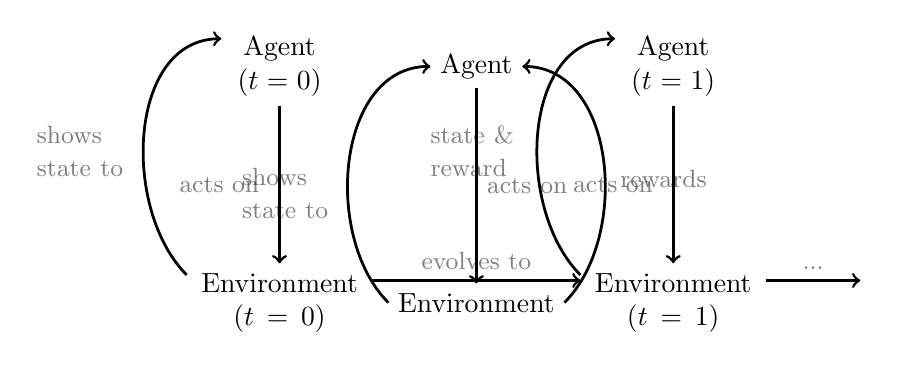
\begin{tikzpicture}[auto]
    \uncover<1-4>{
        \node at (0, 0) (A) {Agent};
        \node at (0, -3) (E) {Environment};
    }
    \uncover<2-4>{
        \path [arrow] (E.west) to [in=180,out=135] node [opacity=0.5, xshift=5pt, yshift=-25pt, text width=40pt] {\small shows state to} (A.west); 
    }
    \uncover<3-4>{
        \path [arrow] (A.south) to  node [opacity=0.5, text width=30pt] {\small acts on} (E.north); 
    }
    \uncover<4>{
        \path [arrow] (E.east) to [in=0,out=45] node [opacity=0.5, xshift=50pt, text width=40pt] {\small rewards} (A.east); 
    }
    \uncover<5-> {
        \node [text width=35pt, align=center] at (-2.5, 0) (A) {Agent (\(t=0\))};
        \node [text width=60pt, align=center] at (-2.5, -3) (E) {Environment (\(t=0\))};
    }
    \uncover<6->{
        \path [arrow] ([yshift=10pt]E.west) to [in=180,out=135] node [opacity=0.5, xshift=5pt, yshift=-20pt, text width=40pt] {\small shows state to} ([yshift=10pt]A.west); 
    }

    \uncover<7->{ 
        \path [arrow] (A.south) to  node [opacity=0.5, xshift=-40pt] {\small acts on} (E.north); 
    }

    \uncover<8->{
        \node [text width=35pt, align=center] at (2.5, 0) (A1) {Agent (\(t=1\))};
        \node [text width=60pt, align=center] at (2.5, -3) (E1) {Environment (\(t=1\))};
    }
    \uncover<9->{
        \path [arrow] ([yshift=8pt]E.east) to node [opacity=0.5] {\small evolves to} ([yshift=8pt]E1.west); 
    }
    \uncover<10->{
        \path [arrow] ([yshift=10pt]E1.west) to [in=180,out=135] node [opacity=0.5, xshift=5pt, yshift=-20pt, text width=40pt] {\small state \& reward} ([yshift=10pt]A1.west); 
    }

    \uncover<11->{ 
        \path [arrow] (A1.south) to  node [opacity=0.5, xshift=-40pt] {\small acts on} (E1.north); 
    }
    \uncover<12>{
        %%\node [text width=35pt, align=center] at (7.5, 0) (A2) {Agent (\(t=2\))};
        \node  at (5, -3) (E2) {};
        \path [arrow] ([yshift=8pt]E1.east) to node [opacity=0.5] {\small ...} ([yshift=8pt]E2.west); 
    }
\end{tikzpicture}
\end{figure}
\end{frame}

\begin{frame}{Agents \& actions}
\begin{columns}
\column{0.5\textwidth}
Agent:
\begin{itemize}
    \item At each time step \(t\), perceives the \textbf{state}, \(s_t\) decides on an \textbf{action}, \(a_t\) from the set of actions available in that state, \(A(s_t)\).
    \item<2-> E.g. press gas, brake, turn wheel left 0.57 radians, press gas + turn right 2.2 radians, shift to 4th gear, ...
\end{itemize}
\column{0.5\textwidth}
    \begin{center}
    \includegraphics[width = \textwidth]{figures/selfdrivingcar.jpg}
    \end{center}
\end{columns}
\end{frame}

\begin{frame}{Environments, states \& transitions}
\begin{columns}
\column{0.5\textwidth}
Environment:
\begin{itemize}
    \item Includes other cars (and also parts of self).
    \item<2-> Is in a state \(s_t\). 
    \item<3-> After the agent takes \(a_t\), evolves to state \(s_{t+1} \in S\) according to the \textbf{transition probabilities}: \(p(s_{t+1} | s_t, a_t)\).
    \item<4-> \textbf{Markov:} transition probabilities depend \emph{only} on \(s_t, a_t\), not history. 
\end{itemize}
\column{0.5\textwidth}
    \begin{center}
    \includegraphics[width = \textwidth]{figures/citystreet.jpg}
    \end{center}
\end{columns}
\note{Sometimes the ``environment'' may include things you intuitively think of as part of the agent, e.g. in the car example the agent would just be the computer, the rest of the car (wheels, etc) would be part of the environment.

So if you're in a state, it doesn't matter how you got to that state} 
\end{frame}


\begin{frame}{Time, \& rewards}
\begin{columns}
\column{0.66\textwidth}
Rewards:
\begin{itemize}
    \item Agent receives a \textbf{reward} \(r_{t+1} \in R\) according to \textbf{reward probabilities}: \(p(r_{t+1} | s_t, a_t, s_{t+1})\). 
    \item<2-> E.g. fare for reaching a destination, penalty for hitting a pedestrian, ...
    \item<3-> \textbf{Return} is the sum of the \textbf{discounted} rewards over time: \(\sum_{t=1}^\infty \gamma^t r_t\) for some \(\gamma \in (0, 1]\).
    \item<4-> \textbf{Discount factor} \(\gamma\) tells how much we prioritize the present over the future.
\end{itemize}
\column{0.34\textwidth}
    \begin{center}
    \includegraphics[width = \textwidth]{figures/money.png}
    \end{center}
\end{columns}
\note{Discounting and the marshmallow task}
\end{frame}

\againframe<12>{mdps}

\begin{frame}[standout]
Questions?
\end{frame}

\section{Learning in MDPs}
\begin{frame}{Policies}
\begin{itemize}
\item How does the agent decide what to do?
\item<2-> By using a \textbf{policy} \(\pi\) which maps states to actions.
\item<3-> This policy could take many forms: picking randomly, a set of rules, a table, a neural network, or some combination thereof.
\item<4-> Ideally, you would want your policy to pick the best action in every state, but what does ``best'' mean?
\end{itemize}
\note{In the case of the car, part of the policy might be ``if you see a pedestrian in front of you, stop, if you can't stop, swerve.'' This might either be implicit or explicit.}
\end{frame}

\begin{frame}{Value functions} 
\begin{itemize}
\item A natural way to define ``best'' states is based on expected return (which we call \textbf{value}). 
    \[V^\pi(s) = \E{\text{Return} \, |\, s} = \E{\sum_{t=1}^\infty \gamma^t r_t \, \bigg \vert \, s } \]
\item<2-> Expectation because this depends on the environment's transistions and rewards, which may be random.  
\item<3-> But this also depends on the policy! (That's why it's \(V^{\color{red} \pi}\).) 
\end{itemize}
\note{expectation of random policy playing chess against me is pretty much always losing, expectation of stockfish's policy is always winning}
\end{frame}

\begin{frame}{Optimality}
\begin{itemize}
\item Now we can define the \textbf{best} policy as the one that gets the \textbf{best} expected return from every state.
\item<2-> We'll denote it by \(\pi^*\) and the associated value function by \(V^*\) or \(V^{\pi^*}\). 
\item<3-> It is a theorem that any problem that can be specified as an MDP has at least one optimal policy.
\item<4-> But how can we try to find \(\pi^*\) or \(V^*\)?
\end{itemize}
\end{frame}


\section{TD Learning and iteration}
\begin{frame}{Chess}
\begin{columns}
\column{0.5\textwidth}
\begin{itemize}
    \item<1-> You're playing chess against Magnus Carlsen. Let's say you estimate that you're doing pretty well, that is \(V^{\pi}(s_t)\) is reasonably high. 
    \item<2-> ... but then he makes a move you don't expect, and you realize you're doing worse than you thought, so \(V^{\pi}(s_{t+1})\) is smaller.
    \item<3-> Can we learn from this difference?
\end{itemize}
\column{0.5\textwidth}
    \begin{center}
    \includegraphics[width = \textwidth]{figures/chess.jpg}
    \end{center}
\end{columns}
\note{How do you think we do it? Well, sometimes you make a move, and then Magnus moves, and then you're like OH I DIDN'T SEE THAT MY POSITION IS MUCH WORSE THAN I THOUGHT.}
\end{frame}

\begin{frame}{TD Learning (applied to chess)}
\begin{itemize}
    \item<1-> Temporal Difference (TD) learning is a formal framework for learning from surprises. 
    \item<2-> For \emph{any} value function, we should have that
        \[V^{\pi}(s_{t}) = r_{t+1} + \gamma V^{\pi}(s_{t+1})\] 
        (This is often called the \textbf{Bellman Equation}.)
    \item<3-> So let's try to make this more true, 
        \[V^{\pi}(s_t) = V^{\pi}(s_t) + \alpha \underbrace{\left( r_{t+1} + \gamma V^{\pi}(s_{t+1}) - V(s_t)\right)}_{\text{prediction error!}}, \quad \alpha \in [0, 1]\]
    \item<4-> Iterating this is guaranteed to converge to the true value function for a policy\footnote{assuming MDP is finite!}.\vspace{3em}
\end{itemize}
\end{frame}

\begin{frame}{TD Learning (in the brain)}

\begin{center}
\includegraphics[height = 0.9\textheight]{figures/dopamine_TD.png}
\end{center}
\end{frame}

\begin{frame}{Actions}
\begin{columns}
\column{0.5\textwidth}
\begin{itemize}
    \item<1-> But even if we have the optimal value function, how do we choose actions? 
    \item<2-> In chess, it's easy -- just look at the next position after you move, and figure out which one has the max value.
    \item<3-> But what about in more complicated situations, where we don't know how the environment will change after our actions?
\end{itemize}
\column{0.5\textwidth}
    \begin{center}
    \only<1-2>{
        \includegraphics[width = \textwidth]{figures/chess.jpg}
    }
    \only<3->{
        \includegraphics[width = \textwidth]{figures/selfdrivingcar.jpg}
    }
    \end{center}
\end{columns}
\note{What do you think?}
\end{frame}

\section{Q-learning}


\begin{frame}{Q-values}
\begin{itemize}
\item The solution we'll explore incorporates the action into our values by estimating the \emph{value of an action in a state}, which we'll denote by \(Q(s,a)\):
    \[Q^\pi(s,a) = \E{\text{Return} \, |\, s, a} = \E{\sum_{t=1}^\infty \gamma^t r_t \, \bigg \vert \, s, a } \]
\item<2-> Notice that this contains the value function from before:
    \[V^\pi(s) = \sum_{a \in A(s)} p(a | s, \pi) Q^{\pi} (s, a)\]
\item<3-> But it also gives us ways of picking policies, e.g. pick the action with the highest \(Q\).
\end{itemize}
\end{frame}

\begin{frame}{Learning Q-values}
\begin{itemize}
    \item<1-> Using TD learning, we have another Bellman equation:
        \[Q^{\pi}\left(s_{t}, a_t\right) = r_{t+1} + \gamma \max_{a'} Q^{\pi}\left(s_{t+1}, a'\right) \] 
    \item<2-> So let's try to make this more true, 
        {\small
        \[Q^{\pi}(s_{t}, a_t) = Q^{\pi}(s_t. a_t) + \alpha \underbrace{\left( \left[ r_{t+1} + \max_{a'} \gamma Q^{\pi}(s_{t+1}, a') \right] - Q(s_t, a_t)\right)}_{\text{prediction error!}}\]}
    \item<3-> Almost surely converges to \(Q^*\) (and by extension \(\pi^*\)), as long as MDP is finite and each state, action pair is visited``enough.'' 
\end{itemize}
\end{frame}

\begin{frame}[standout]
Questions?
\end{frame}

\begin{frame}{Wrapping up}
\begin{itemize}
    \item Audience participation!
    \begin{center}
        \includegraphics[width=0.3\textwidth]{figures/walkingbaby.jpg}~
        \includegraphics[width=0.3\textwidth]{figures/selfdrivingcar.jpg}~
        \includegraphics[width=0.3\textwidth]{figures/playingchess.jpg}
    \end{center}
    \item<2-> Are there potential problems with what we've learned so far?
    
\end{itemize}
\note{AP: Identify the things we've learned in each of these tasks}
\end{frame}


\end{document}
